\chapter {DASAR TEORI}

Pada bab ini, akan dijelaskan dasar teori yang digunakan sebagai landasaan pengerjaan Tugas Akhir ini.

\section{Deskripsi Permasalahan}
Permasalahan yang dibahas pada Tugas Akhir ini adalah perhitungan untuk mencari perimeter poligon terkecil dari sekumpulan titik yang dibatasi di dalam poligon sederhana.\cite{isun1}
\begin{figure}
	\Centering
	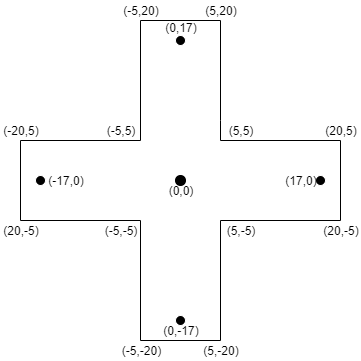
\includegraphics [width=0.5\columnwidth]{bab2/img/contoh-kasus-tanpa-solusi}
	\caption {Ilustrasi contoh kasus tanpa solusi}
	\label {fig:ilustrasi-contoh-kasus-tanpa-solusi}
\end{figure}
\begin{figure}
	\Centering
	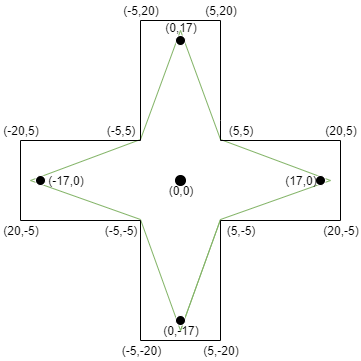
\includegraphics [width=0.5\columnwidth]{bab2/img/contoh-kasus}
	\caption {Ilustrasi contoh kasus}
	\label {fig:ilustrasi-contoh-kasus}
\end{figure}

\section{Strategi Penyelesaian Permasalahan}
Pada buku ini hanya membahas poligon pembatas hanya terbentuk dari poligon sederhana. Titik yang berada di dalam poligon tersebut dapat diganti dengan poligon sederhana, segment garis atau yang lainnya.
\par Asumsikan poligon $A$ mempunyai $n$ vertex, dimana $A = \left \langle a_1, a_2, ..., a_n \right \rangle$. Poligon $A$ merupakan poligon yang membatasi kumpulan titik $S$ yang mempunyai titik sebanyak $m$ ($S = \left \langle s_1, s_2, ..., s_m \right \rangle$). $D(A)$ merupakan sebuah deque yang menampung vertex dari poligon $A$.
\par untuk setiap 

\section{Melkman Convex Hull Algorithm}
Merupakan algiritma untuk menghitung rantai poligonal atau poligon sederhana dengan waktu linear ($O(n)$)\cite{melkman_algorithm}. Asumsikan sebuah rantai poligonal $C = (v_0, v_1, ..., v_{n-1})$, dengan vertex $v_i$ dan edge $v_i v_{i+1}$. Algoritma ini menggunakan deque (\textit{doubly-ended queue}), $D = \left \langle d_1, d_2, ..., d_n \right \rangle$, untuk mereprentasikan \CH, $Q_i = CH(C_i)$, dimana $C_i = (v_0, v_1, ..., v_i)$. Deque mempunyai fungsi \textit{push} dan \textit{pop} dari atas/depan dan \textit{insert} dan \textit{remove} dari bawah/belakang. Secara spesifiknya yang dilakukan \textit{push} $v$ ke deque melakukan $(l \leftarrow l+1; d_t \leftarrow v)$, untuk \textit{pop} $d_t$ dari deque melakukan $(t \leftarrow t-1)$, untuk insert $v$ ke deque melakukan $(b \leftarrow b-1; d_b \leftarrow v)$, dan \textit{remove} $d_b$ dari deque melakukan $(b \leftarrow b+1)$.
\par Algoritma ini menggunakan konvensi dimana vertexnya berurutan secara berlawanan jarum jam di sekitar \CH $Q$.
\par Setiap $d_t$ dan $d_b$ mengacu kepada vertex yang sama pada rantai poligon $C$, dan vertex ini akan selalu menjadi vertex yang kita tambahkan terakhir pada \CH.
\begin{figure}
	\Centering
	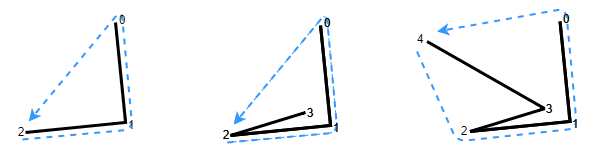
\includegraphics [width=\columnwidth]{bab2/img/ilustrasi-algoritma-melkman}
	\caption {ilustrasi algoritma melkman}
	\label {fig:ilustrasi-algoritma-melkman}
\end{figure}
\begin{algorithm}
	\caption{Melkman Convex Hull}
	\label{psdo:Melkman Convex Hull}
	\begin{algorithmic}[1]
		\Require $C$
		\Ensure $Q$
        \State Inisialisasi: $D$
        \If{Left($v_0, v_1, v_2$)}
            \State$D \leftarrow \left \langle v_2, v_0, v_1, v_2 \right \rangle$
        \Else
            \State $D \leftarrow \left \langle v_2, v_1, v_0, v_2 \right \rangle$
        \EndIf
        \State $i=3$
        \While{$i<n$}
            \While{ Left($d_{t-1}, d_t, v_i$) dan Left($d_b, d_{b+1}, v_i$))} 
                \State $i \leftarrow i+1$
            \EndWhile
            \While{!Left($d_{t-1}, d_t, v_i$)}
                \State \textit{pop} $d_t$
            \EndWhile
            \State \textit{push} $vi$
            \While{!Left($v_i,d_{b}, d_{b+1}$)}
                \State \textit{remove} $d_b$
            \EndWhile
            \State \textit{insert} $vi$
            \State $i \leftarrow i+1$
        \EndWhile
	\end{algorithmic}
\end{algorithm}

\section{Algoritma Monotone Chain}
Algoritma \MC merupakan proses pembentukan \CH dari sekumpulan titik dengan kompleksitas $O(n$ log$(n))$\cite{monotone_chain_algorithm}. Asumsikan sekumpulan titik $S$ sejumlah $n$ ,$S = \left \langle s_1, s_2, ..., s_n\right \rangle$ algoritma ini menggunakan list untuk membentuk sebuah rantai (\textit{monotone chain}), dimana list $L(S)$ menampung semua titik yang ada di $S$ yang terurut berdasarkan nilai koordinatnya terhadap sumbu $x$. algoritma ini memeriksa setiap 3 vertex yang berurutan, jika 3 vertex tersebut membuat convex makan ketiga vertex tersebut disimpan, dan sebaliknya jika ketiga vertex tersebut membuat concave maka vertex ke 2 akan dibuang dari vertex penyusun convex hull. lalu lakukan hal yang sama dengan membalikan urutan pada $L$ untuk mendapatkan \textit{lower hull}.

\begin{figure}
	\Centering
	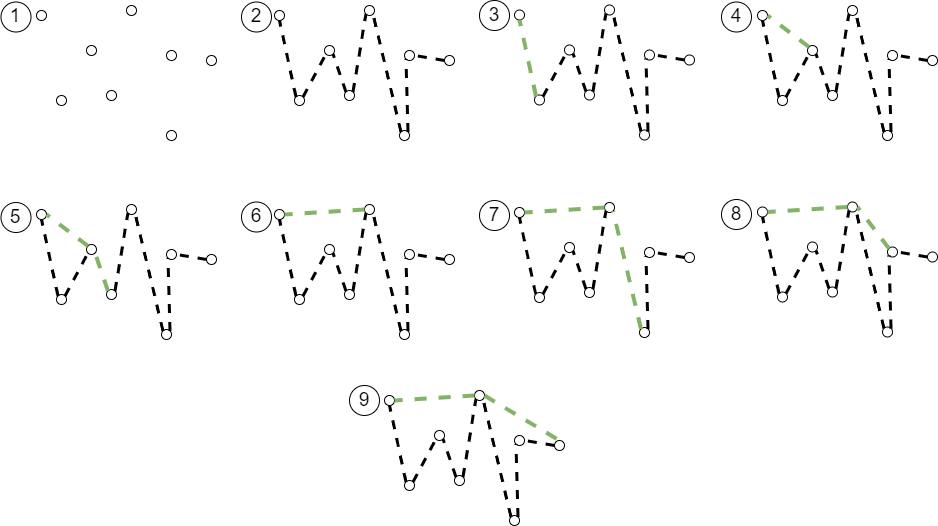
\includegraphics [width=\columnwidth]{bab2/img/ilustrasi-algoritma-monotone-chain}
	\caption {Ilustrasi algoritma monotone chain}
	\label {fig:ilustrasi-algoritma-monotone-chain}
\end{figure}

\begin{algorithm}
	\caption{Monotone Chain Algorithm}
	\label{psdo:Monotone Chain Algorithm}
	\begin{algorithmic}[1]
		\Require $S$
		\Ensure $CH(S)$
        \State Inisialisasi: $L$
        \State Sort $S$
        \State $L \leftarrow S$
        \State Inisialisasi $CH(S)$
        \For{$i=0;i<2;i++$}
            \For{$j=0;j<Size(L);j++$}
                \While{$Size (CH)\ge2$ and $right(CH[Size(CH)-1],CH[Size(CH)-2],S[j])$}
                    \State Delete $CH$ last element
                \EndWhile
                \State push $pt$ to $CH$
            \EndFor
            \State reverse $L$
        \EndFor
	\end{algorithmic}
\end{algorithm}
\section{POint Inside Polygon}
blalasjbfkljawegfbawefe \cite{point_inside_polygon}